\documentclass[11pt]{article}
\usepackage{fullpage}
\usepackage{epstopdf}
\usepackage{titlesec}
\usepackage{amssymb,amsmath}
\usepackage{amsthm}
%\usepackage{subfigure}
\usepackage{subcaption}
\usepackage{graphicx}
\usepackage[]{algorithm2e}
\usepackage{xcolor,listings}
\usepackage{multirow}
\usepackage{hyperref}
\usepackage{varwidth}
\newtheorem{thm}{Theorem}

\setcounter{secnumdepth}{4}
\titleformat{\paragraph}
{\normalfont\normalsize\bfseries}{\theparagraph}{1em}{}
\titlespacing*{\paragraph}
{0pt}{3.25ex plus 1ex minus .2ex}{1.5ex plus .2ex}

\title{LCH: A Reliable Distributed Source Code Version Control System}
\author{Shike Mei, Menghui Wang, and Lichao Yin}

\begin{document}
\maketitle

\abstract{
    Today popular source code version control systems do not replicate data for reliability.
    We share our experience in building LCH (abbreviated from Launch), a reliable source code version control system.
    LCH replicates data on multiple servers and uses the Paxos\cite{paxos} protocol along with an update log to provide strong consistency to clients.
    With a three-step catch-up mode, LCH can also recover from failures seamlessly.
    Our test results show LCH is a reliable version control system.
}

\section{Introduction}

A version control system is a system that keeps track of multiple history versions of every managed document, and allows a user to checkout or revert to previous versions as needed.
Version control systems usually allow for a group of people contributing to one project.
Today version control systems have an extensive use in source code management, collaborative editing, data backup, etc.

Due to different applications, a version control system can differ from another in many aspects.
\begin{itemize}
    \item History granularity: linear versus directed acyclic graph (DAG).
        Examples include: Google Docs (linear), Subversion (linear), git (DAG), Mercurial (DAG).
    \item Implicit checkpointing versus explicit checkpointing.
        An implicit checkpointing system will automatically save the state of the current document whenever the system thinks appropriate, while an explicit checkpointing system will not do so until instructed by the user.
        Examples include: Google Docs (implicit), Dropbox (implicit), git (explicit), Subversion (explicit).
    \item Conflict Resolution.
        A conflict is when multiple versions of a same file (or a same line of a same file) are found at the same time.
        Conflicts could result from out-of-date repository, conflicting edits from different sources, network delays, or system faults.
        Some systems will resolve conflicts automatically based on some metrics or mechanisms.
        Some examples include conflict resolution by timestamp (Google Contacts), vector clocks.
        Other systems will need human intervention to resolve conflicts (Dropbox, git, Subversion, CVS).
    \item Failure model.
        Some systems have a centralized server and thus are vulnerable to single-node failures (Subversion, CVS, git, Mercurial\footnotemark),
        while others will store data reliably on a distributed set of servers (Google Docs).
        \footnotetext{
        Although git and Mercurial are capable of storing data on multiple servers, replication is not supported natively and users will need to push data to every single place manually.
        Moreover, since atomicity is not provided when doing so, it may will cause complex consistency issues.
    For this reason, most git and Mercurial users will use git and Mercurial in the same way as they use Subversion: designate a central server to store all the data.}
    \item Offline edits.
        Some systems allow making modifications while offline (git, Dropbox) while others do not (Subversion, Google Docs).
\end{itemize}

Replication is the key to reliability.
However from the list above one can see that today few version control system replicates data.
This motivates our project.
Simply speaking, LCH is a version control system that will store source code reliably on a distributed set of servers.
Source code is different from other application in that it needs to be precise at any time.
Thus strong consistency needs to be preserved while replicating data.
Paxos\cite{paxos} is a protocol that solves the consensus problem in a distributed system.
With the help of an update log, we can build a strongly consistent distributed system that replicates data across many servers.

LCH is designed to tolerate failures.
When a failed server is restarted, it will first operate in a 3-step catch-up mode.
Unlike the catch-up mode proposed by Google \cite{paxos2}, we add an additional third step that will make sure everything missed out is collected.
The catch-up mode will be discussed in detail in Section~\ref{sec:impl}.

In the original protocol, it is possible that Paxos rounds keep failing because multiple proposers make conflicting proposes in an alternating way.
We propose random backoff to mitigate this issue.
In our solution, when such scenario is detected, a proposer will, with a certain probability, try to postpone its proposal for a random period of time, so as to minimize the likelihood that more than one proposers propose at the same time.

In the rest of this paper we discuss the various trade-offs in when we design LCH, and we share our experience in implementing it.
It is organized as follows: in Section~\ref{sec:design}, we discuss our reasonings and considerations behind the various decisions we made in designing LCH.
Section~\ref{sec:impl} will mainly focus on implementation details of the server and the client, including how we incorporate the Paxos protocol in our system and some improvements of it.
Section~\ref{sec:eval} will state our methodology in evaluating our system.
Section~\ref{sec:conclusion} concludes our project.


\section{Design}
\label{sec:design}
In this section we will discuss the design of LCH, as well as our reasonings behind every decision.

\subsection{System Overview}
LCH is a client-server application.
Unlike a traditional version control system, user data is replicated on multiple LCH servers for reliability.
Figure~\ref{fig:1} shows a typical topology structure of LCH.

\begin{figure}[ht!]
\centering
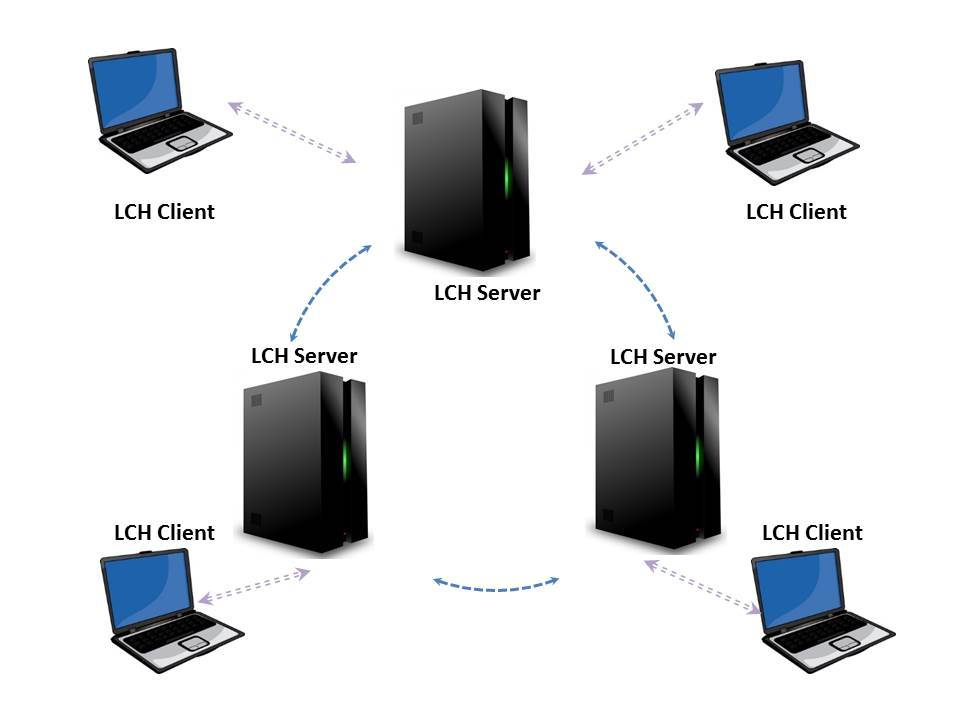
\includegraphics[width=110mm]{architecture.jpg}
\caption{Architecture of LCH}
    \label{fig:1}
\end{figure}

\subsection{Distributed Servers}
LCH is a distributed system.
Multiple servers can serve their own clients in the same time.
Every client can choose to connect to any LCH server, and servers will handle replication and consistency behind the scene.
Client will feel like there is only one server there.
That being said, when the server a client is connecting to is not responding, the client can choose to connect to any other server.
In contrast to our distributed design, an alternative is to use a master-slave scheme.
Although the master-slave scheme handles consistency issues more easily, it is less reliable than our distributed structure.
For example, when a master failure is monitored, a master flip must be done.
During the flip, there is a short period of time that the system is not available.
Moreover, a master failure may also cause data loss.

\subsection{Client Design}
LCH uses similar terminologies and concepts as were used in other version control systems.
A version is a state consisting of the states of all managed files.
Changes made to a version are called a commit, and a commit will lead to a new version.
LCH provides linear version history, which means commits can only be made to the latest version.
As a consequence, every version is associated with a single integral number, beginning from $0$, which is the version for an empty repository.
It is worth noting that although we choose to implement LCH using linear version history, DAG version history can also be achieved under our design.
We choose to use linear version history because it provides a cleaner and more understandable interface to the user, and it is less likely for misoperations to happen.
Though a DAG-based history is more powerful and flexible, it is also harder to implement and we choose not to spend our efforts on it.

The client offers two simple commands, \texttt{sync} and \texttt{commit}.
\texttt{sync} will pull from a server recent changes from the current version of the client, and then the client will apply all those changes.
A \emph{conflict} may happen when both remote and local changes are made to the same file.
In this case, the remote change will not be applied, and a copy of the remote file will be created.
Then the user will be directed to resolve the conflict.
We choose to let the user to resolve conflicts for the following two reasons:
\begin{itemize}
    \item The conflicts happen in LCH are not easily resolvable by a machine or by certain rules.
        A conflict usually involves two uncomparable versions due to modifications made on an outdated repository.
        Consolidating them requires knowledge beyond the scope of the system.
    \item Human has a better understanding of what the code is doing, and is more capable of resolving conflicts.
\end{itemize}

\texttt{commit} command will scan the all the local files, and compute the changes made to the current local version.
Then it will push these changes to the remote server.
There are two possible outcomes: accepted or rejected.
If the commit is accepted, then the local version is advanced by $1$.
Otherwise, it must be because the local version is out-dated.
Thus the user must run the \texttt{sync} command first.
The main reason LCH uses explicit checkpointing is that we feel it is better to let user to organize each commit because user has a better understanding of what the code does.

\subsubsection{Online Commits}
LCH requires that all commits must be submitted to servers at the time they are made.
Therefore no offline commits are allowed.
This is a consequence of our previous designs,
\begin{itemize}
    \item Since it is possible that a commit be rejected by the server, the client must contact the server to know if this is the case.
    \item If we allow a commit to be staged but not submitted, it will cause more consistency issues.
        Suppose one of the staged commit turns out to be rejected by the server.
        What should we do to its following commits?
        There is no easy way we can handle this under our linear history model.
\end{itemize}

\subsubsection{A Typical Workflow}
Figure~\ref{fig:2} shows a typical use case of LCH.
The user first run a \texttt{sync} command to sync its local repository.
The user then make modifications to its local repository until it is ready for a checkpoint.
Then a \texttt{commit} command will be run, and the client will notify if the commit is accepted or not.
If the commit is accepted, the user can keep making other changes.
Otherwise, the user must run a \texttt{sync} command to pull latest changes from the server.
Conflicts may happen during this step, and if this is the case, the user must resolve conflicts given the remote file and the local file.
When conflicts are resolved, the user can run another \texttt{commit} command to submit previous changes (along with the conflict resolution).

\begin{figure}[ht!]
    \centering
    \begin{varwidth}{\textwidth}
\begin{enumerate}
    \item Initialization
    \item Make changes
    \item \texttt{sync}
    \item Resolve conflicts
    \item \texttt{commit}
    \item Accepted? Goto step $2$; otherwise goto step $3$.
\end{enumerate}
\end{varwidth}
\caption{A typical workflow}
    \label{fig:2}
\end{figure}


\subsection{Full Replication}
Every LCH server is identical and equally capable.
This means, every LCH server will store a whole database of all history commits.
We do not choose to partition our data for the following reasons:
\begin{itemize}
    \item Full replication provides higher read throughput than partitioning does.
        In our current design, every server is able to serve sync requests clients in parallel
        (not true for commit requests because they need to go through a Paxos round).
        If we partition our data, every server will only be able to serve requests concerning the portion of data it has.
    \item As for a version control system for source code, it is unlikely that the size of a single repository will exceeds the limit of a single machine.
        Therefore there is no need to replicate data for capacity as well.
\end{itemize}

\subsection{Strong Consistency}
When designing our consistency model, our criteria is ``every commit submitted must base on the things that the user has already \emph{seen}'', because source code must be precise at all times.
Therefore we choose to maintain strong consistency and let user to resolve conflicts.
That is, every \texttt{sync} command will return the latest version by a most recent \texttt{commit}, and no commit shall be accepted unless it is based on the latest version.

Strong consistency is at the cost of reduced throughput.
To preserve strong consistency, every commit must go through a full Paxos round, which will involve all servers to participate.
As a result, only one commit will be accepted at a time among all servers.
However, as a tool for managing source code, we do not anticipate a very high concurrent commit rate.

\subsection{Fault-Tolerant and Recovery}
LCH tolerates non-Byzantine failures by replication.
When a server failed, since all the servers are equally capable, the client can choose to connect to any other servers with the same request.
As long as the total number of failed servers is less than half of the total, LCH will work normally.
This result is implied by the fault-tolerant characteristic of the Paxos protocol.
To see rigorously how replication improves the reliability, one can refer to Theorem~\ref{thm:1} in Appendix.

When a failed server is restarted, it must start in a catch-up mode.
The catch-up mode will help the failed server catch up all the information it missed during failures.
They are essentially the results of previous Paxos rounds.
Before it can serve in normal mode again, it must ensure that the data stored on it is synchronized with every other sever.
We will discuss the techniques used in the catch-up mode in detail in Section~\ref{sec:impl}.

\section{Implementation}
\label{sec:impl}
In this section we will discuss various implementation details when we build LCH.
We coded LCH from scratch in Java and the source code is available online\footnotemark.
\footnotetext{\url{https://github.com/kirakira/lch}.}

\subsection{Paxos and Update Log}
\label{sec:paxos}
Paxos is a consensus protocol introduced in \cite{paxos}.
It solves the following problem:
every server has its own proposal, and the group of servers want to agree on one of the proposals.
In LCH, every server will store a database containing all the accepted commits, and the database stored in every server should all be identical.
The Paxos protocol is used to select a request to modify the database.
Since all servers run in parallel, it is possible that at the same time multiple servers have received commit requests.
By our consistency requirement, only one commit can be based on the current version.
Then which commit request should we process?
This is when the Paxos protocol comes into play.
We will use the Paxos protocol to make all servers agree on one commit request to \emph{process}.

Though we select one commit request globally, the selected request is then being processed locally with the help of the update log.
The update log contains the results of all previous Paxos rounds, i.e. all the commits that were selected to process (but not necessarily to accept due to the existence of out-of-date commits).
After a Paxos round finishes, a new entry is first being added to the update log carrying the result of this Paxos round.
The newly added entry is marked as ``unfinished'' at this time.
It is first decided, according to the server's local database, whether this commit should be accepted based on the following criteria: if this commit is based on the current version, then it should be accepted; otherwise it should not.
If it is decided that the commit should be accepted, the server then applies the commit in the database.
Finally, the server modifies the corresponding entry in the update log to change its state to ``finished''.
If the current server happens to be the server that received the request, it will then notify the client the result of this commit.

\subsubsection{Implementation Details}
The original Paxos protocol has $3$ roles: proposer, acceptor, and learner.
We combined the latter two roles, and used $2$ threads each server doing the Paxos logic.
One thread will listen to client's \texttt{commit} requests and acts as the proposer.
The other thread will act as the acceptor and learner.

A global condition variable \texttt{roundFinish} will be used to synchronize the two threads.
\texttt{roundFinish} will be signaled by the acceptor and learner thread when a Paxos round has finished.

The activity of a proposer is initialized by an incoming commit request.
Only one commit request will be processed at the same time.
The proposer will first select a unique proposal number higher than any previous proposal numbers as follows:
it selects an integer $x$ greater than any previous proposal numbers and such that $x \equiv i \mod n$ where $n$ is the total number of proposers and $i$ is the $0$-based index of the current proposer.
It then starts to make proposals to every server (including itself) as specified by the Paxos protocol.
After all accept requests are sent out, it sleeps on the condition variable \texttt{roundFinish}, waiting for the result to be notified by the learner thread.
After being waken (or timed out after $10$ seconds), it checks the database to see if the request commit has been applied or not.
If everything goes well, the commit should pass the Paxos round and be learned by the learner thread (by writing to the update log and the database)
Finally the proposer will notify the result (accepted or not) to client.

The activity of the acceptor and learner thread is initialized by incoming Paxos packets (prepare, accept request, accepted, rejected).
The thread is implemented as a state machine, where the state includes the most recent promise \texttt{promise} made in this round, and the highest numbered proposal accepted \texttt{accepted}.
A round is regard as finish when more than half ``accepted'' are received for some proposal.
When a round is finished, \texttt{promise} and \texttt{accepted} are first cleared, and then the update log and the local database is updated atomically if necessary according to the selected commit request as is specified in \ref{sec:paxos}.
Finally, the condition variable \texttt{roundFinish} is signaled to wake all proposers sleeping on that.

\subsection{Catch-up Mode}
When a server is back from failure, it cannot start to serve immediately because of its out-of-date update log and database.
To get synchronized with the latest state, it executes in catch-up mode.

\begin{enumerate}
    \item At the first step, the server will do an anti-entropy pull of update log from another server.
        Since every server operating in normal mode must have latest database and update log, it suffices to pull from one server.
    \item Then it participates in a full Paxos round as an observer.
        This means,
        \begin{itemize}
            \item It will observe the round and learn the results of this round.
            \item But it cannot vote or propose.
        \end{itemize}
        This Paxos round is necessary for the following reasons:
        \begin{itemize}
            \item It needs to know the current largest proposal number.
                This number will be used for future proposals.
            \item It needs to make sure that it has grabbed the latest update.
            \item It needs to make sure it be in the start of a new Paxos round when back in the normal mode, not in the middle of a ongoing Paxos round.
        \end{itemize}
    \item Finally another anti-entropy pull is done to collect all updates happened between step $1$ and step $2$.
        This step is also necessary.
        Consider for example the server started step $2$ in the middle of an ongoing Paxos round.
        It is very likely that the server will only receive part (less than half) of the ``accpeted'' votes while actually all servers voted ``accepted'' (the votes the current server missed were delivered before the current server started step $2$).
        Consequently the current server will not consider this as a successful Paxos round, while other servers will because other servers have received all ``accepted'' votes.
        As a result, the current server will not learn the result.
        This missed result will need to be collected in step $3$.
\end{enumerate}
The above catch-up mode is different from the catch-up mode introduced in \cite{paxos2} in that it adds a third step that will collect all updates missed during the execution of the first and the second step.

\subsection{Random Backoff}
The traditional Paxos protocol may not make any progress when two or more proposers make conflicting proposals alternately,
as is noted in \cite{paxos}.
The random backoff protocol is a randomized solution that can mitigate this issue.

Intuitively, a Paxos round will fail because too many proposers are proposing in the same time.
Thus our goal is to restrict the number of proposers, and the interleave the time they propose.
To be precise, when a failed Paxos round is detected (that is, when multiple proposers are proposing and more than half of the ``rejected'' votes are received for both proposal),
random backoff process will be triggered.
The server will with probability $1-1/k$ stop proposing for $t$ seconds, where $k$ is the number of active proposers detected, and $t$ is selected uniformly at random from a preconfigured time interval.
Note that $1-1/k$ is chosen in a way that will maximize the probability that exactly one proposer will keep proposing
(as a necessary condition, one can check that the expected number of proposers that will keep proposing is $k\left(1-\left(1-1/k\right)\right)=1$).

\subsection{Client}

The client will store a list of remote servers.
Each request will be routed to a randomly chosen server from the list, in case failures happen.
In addition, a metadata folder will be created.
This folder will contain all history commits.
For each commit, we store the difference of each changed file from the last version.

When processing a \texttt{sync} command, a sync request enclosed with the current local version number is sent to a randomly chosen server from the server list.
The server will respond with a list of commits since the current local version.
Then we compare every local local change with its corresponding remote change to detect for conflicts.
If a conflict is found, it will be reported and its corresponding remote version of the file will be saved as a temporary file for the user to resolve the conflict.
If a file is not in conflict, then it is updated to the latest version automatically.
Finally, the metadata file and the local version number is updated to reflect the latest remote version as returned by the server.

When processing a \texttt{commit} command, we scan the current folder for all changes made, based on the latest version stored in the metadata file.
Then a commit request is sent to a randomly chosen server along with the current local version number and all the local changes made.
If the server responds ``accept'', the local version number is updated.
Otherwise, depending on the reason of failure, either the client will retry if the commit is rejected because of a failed Paxos round, or the user will be directed to run the ``sync'' command if it is because out-of-date local repository.

\section{Evaluation}
\label{sec:eval}
We evaluated the correctness and performance of our implementation.
The correctness test mainly focuses on the Paxos protocol and the catch-up mode.
The performance test reveals the relationship between the average commit latency and the number of servers.

\subsection{Consistency Test}
We set up $10$ servers and $10$ clients.
This test consists of several rounds.
In each round, all the clients submit a commit request to its corresponding server (i.e. client $0$ contacts server $0$, client $1$ contacts server $1$, etc.) at the same time.
Since Paxos should select at most $1$ commits to process, we expected at most $1$ commit will be accepted.

Our results show that in $9$ out of $10$ rounds exactly $1$ commit is accepted, and in the rest round no commits are accepted due to Paxos round failure.

\subsection{Reliability Test}
We set up $3$ servers and $1$ client.
We make the client keep submitting random commits.
In the meanwhile, we turned down one of the servers.

We observed that although the average latency of commits has increased significantly (because when the commit is submitted to the failed server, the client needs to wait until timeout), commits are still being accepted as they should be.

\subsection{Catch-up Mode Test}
After the reliability test, we restarted the server that we turned down previously in catch-up mode, while the client is still submitting random commits.
It is observed that after a while, the average latency went to normal level again.

\subsection{Latency Test}
We tested the average latency of commit requests.
We first set up $n$ servers on the local machine (so as to minimize network latency), and make a local client submit $100$ commits sequentially.
Then we measure the total time used.
Since a Paxos round with $n$ servers will communicate $O(n^2)$ messages, we expect the average latency will increase with the number of servers.
In practice this is not a problem because usually $n$ is chosen to be fairly small, i.e. $n=3$ or $n=5$.

Results of the latency test are summarized in Table~\ref{tab:perf} and Figure~\ref{fig:perf}.
\begin{table}[ht!]
    \center
\begin{tabular}{c|ccccc}
    \hline
    \hline
    Number of servers & $3$ & $5$ & $7$ & $9$ \\
    \hline
    Average commit latency (ms) & $21.97$ & $36.49$ & $60.17$ & $77.63$ \\
    \hline
    \hline
\end{tabular}
\caption{Average commit latency with different number of servers}
\label{tab:perf}
\end{table}

\begin{figure}[ht!]
\centering
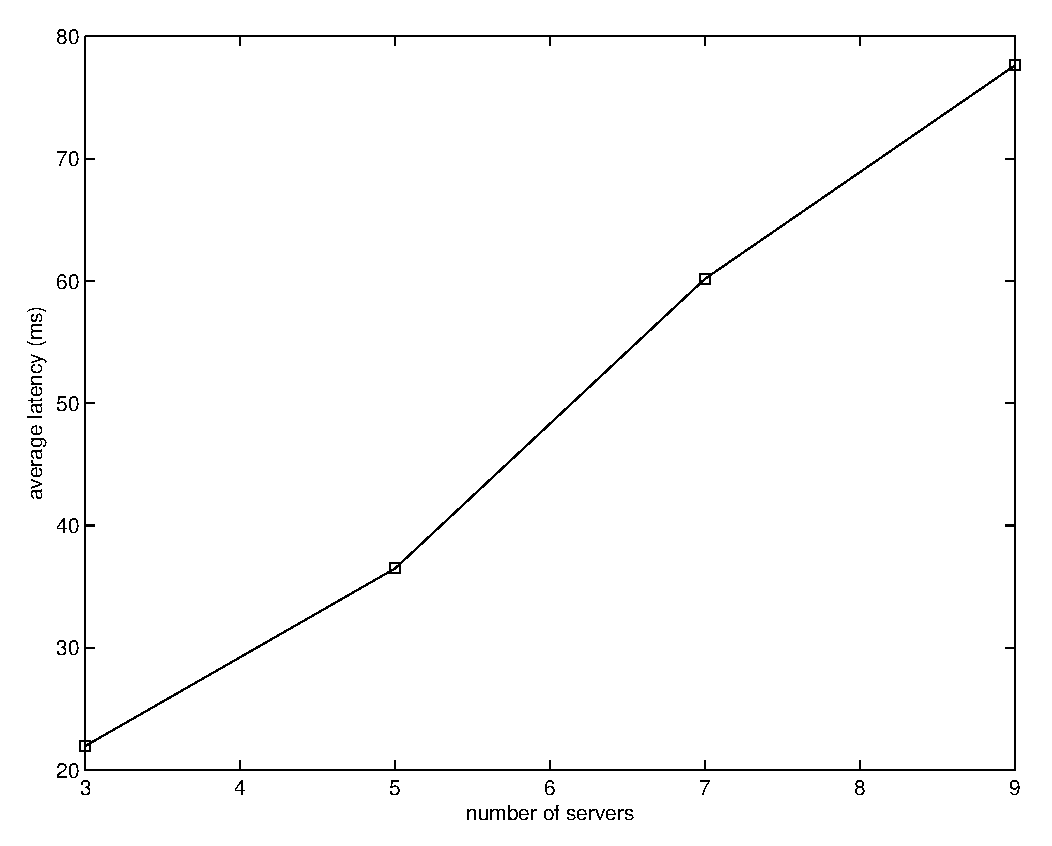
\includegraphics[width=12cm]{perf.eps}
\caption{Average commit latency with different number of servers}
\label{fig:perf}
\end{figure}

\section{Conclusion}
\label{sec:conclusion}
This project demonstrates LCH, a reliable source code version control system by replicating data on multiple servers.
It uses the Paxos protocol along with an update log to maintain strong consistency.
It features a $3$-step catch-up mode to make failed servers recover from failures seamlessly.
The random backoff protocol also makes the Paxos round more efficient when many proposers are proposing conflicting values.
Our evaluations show LCH has met all its design expectations.


\appendix
\section{A Proof that Replication Improves Reliability}
\begin{thm}
    \label{thm:1}
    Assuming that each server fails independently with probability $p$ $(p<0.5)$.
    If there are $2n+1$ servers, then the probability that more than $n$ servers fail simultaneously is less than $p$.
\end{thm}
\begin{proof}
    Let $S \subset \left\{1,\ldots,2n+1\right\}$ be the set of failed servers.
    The probability that $m$ out of $2n+1$ servers fail simultaneously (denote as $\Pr(|S|=m)$) is 
    \begin{eqnarray*}
        \Pr(S=m) = \binom{2n+1}{m} p^{m} (1-p)^{2n+1-m},
    \end{eqnarray*}
    where $\binom{2n+1}{m}$ is the binomial coefficient.
    The probability that more than $n$ servers fails is denoted as $\Pr(|S|\geq n+1)$.
    \begin{eqnarray*}
        \Pr\left(|S|\geq n+1\right) = \sum_{m=n+1}^{2n+1} \binom{2n+1}{m} p^{m} (1-p)^{2n+1-m}.
    \end{eqnarray*}
    To prove that $\Pr(|S|\geq n+1) < p$, we first show prove that $\Pr(|S|\geq n+1)/p = 1$ 
    when $p=1/2$. It is because
    \begin{eqnarray*}
        \Pr(|S|\geq n+1) &=& \sum_{m=n+1}^{2n+1} \binom{2n+1}{m} p^{m} (1-p)^{2n+1-m} \\ 
        (because~p=1/2)~&=& \sum_{m=n+1}^{2n+1} \binom{2n+1}{m} \left(\frac{1}{2}\right)^{2n+1} \\
        \left(because~\binom{2n+1}{m}=\binom{2n+1}{2n+1-m}\right)~&=& \frac{1}{2}\left(  \sum_{m=0}^{2n+1} 
        \binom{2n+1}{m} \left(\frac{1}{2}\right)^{2n+1} \right) \\
        &=& \frac{1}{2}.
    \end{eqnarray*}
    We then prove that the $\Pr(|S|\leq n+1)/p$ is monotonously increasing with as $p$ 
    increasing (and $p<1/2$) by showing the derivative with respect to $p$ is positive
    \begin{eqnarray*}
        \frac{\mathrm{d}}{\mathrm{d}p}\Pr(|S|\geq n+1)/p &=& \sum_{m=n+1}^{2n+1} \binom{2n+1}{m} \left(\left(m-1\right)p^{m-2}
        \left(1-p\right)^{2n+1-m} \right.\\
        &&\left. - \left(2n+1-m\right)p^{m-1}\left(1-p\right)^{2n+1-m-1}\right) \\
        &=& \sum_{m=n+1}^{2n+1} \binom{2n+1}{m} \left(p^{m-2} 
        \left(1-p\right)^{2n+1-m-1}\left(m-1-2np\right)\right)\\
        (because~m-1-2np>0)&>& 0.
    \end{eqnarray*}
    So $\Pr(|S|\geq n+1)/p$ is increasing with $p$ when $p<0.5$.
    Since $\Pr(|S|\geq n+1)/p=1$ when $p=1/2$ and for $p<1/2$, $\Pr(|S|\geq n+1)/p$ is 
    increasing, $\Pr(|S|\geq n+1)/p < 1$ for all $p<1/2$. Therefore, the probability 
    that more than $n$ out of $2n+1$ servers fail simultaneously is smaller than 
    $p$.
\end{proof}

\bibliography{refs}{}
\bibliographystyle{plain}

\end{document}
